\documentclass[../../main.tex]{subfiles}
\begin{document}

\section{Medici\'on corriente de bias y tensi\'on de offset}

\subsection{Importancia de las corrientes de bias y la tensi\'on de offset}



\begin{figure}[htb]	%modelo opamp vio ibias
	\centering
	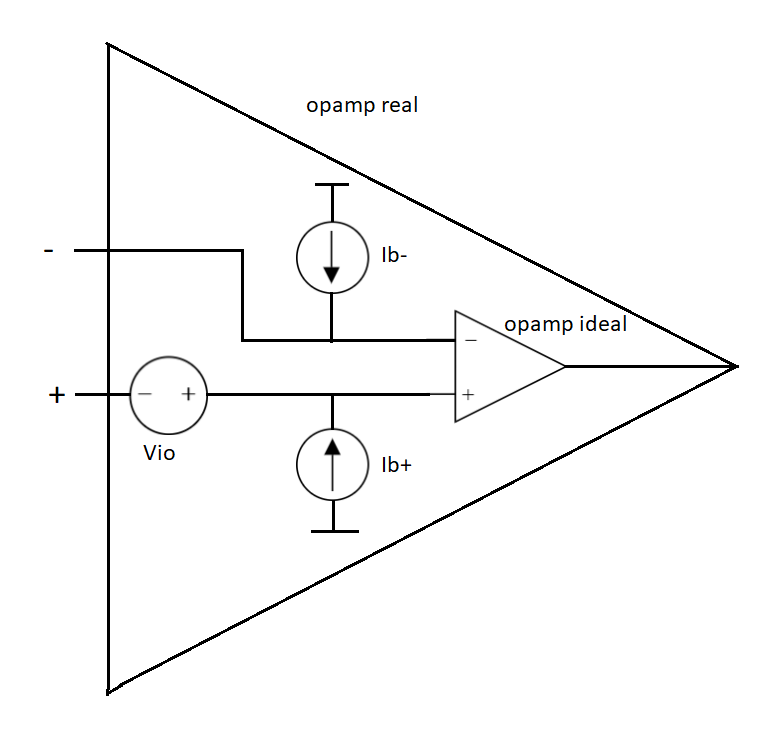
\includegraphics[width=0.7\textwidth]{imagenes/modelo_opamp_vio_ibias.png}
	\caption{Modelo de amplificador operacional con corrientes de bias y tensi\'on de offset}
	\label{fig:ej_3_modelo_opamp_vio_ibias}
\end{figure}






Las corrientes de bias($I_B^+$ y $I_B^-$) y la tensi\'on de offset ($V_{IO}$) pueden generar efectos que no concuerdan con el modelo ideal de un amplificador operacional. Se presentan a continuaci\'on tres ejemplos:

\subsubsection*{Efecto de $V_{IO}$}

\begin{figure}[htb]	%vio no despreciable
	\centering
	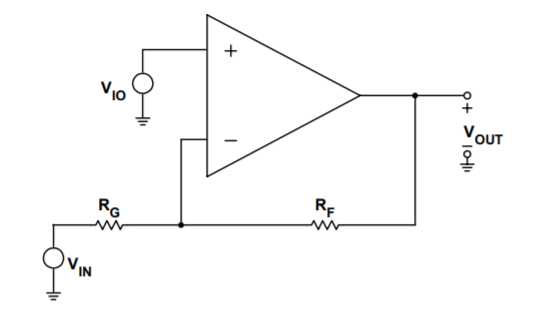
\includegraphics[height=0.2\textheight]{imagenes/vio_amplificacion.png}
	\caption{Amplificador con $V_{IO}$ no despreciable en configuraci\'on inversora }
	\label{fig:ej_3_efecto_vio}
\end{figure}

El circuito de la figura \ref{fig:ej_3_efecto_vio} representa un amplificador operacional en configuraci\'on inversora con tensi\'on de offset no despreciable modelado por un \textit{op-amp} ideal y una fuente de tensi\'on continua $V_{IO}$. De ignorarse la tensi\'on de offset, puede obtenerse la funci\'on transferencia:

\[\frac{V_{OUT}}{V_{IN}}=\frac{-R_F}{R_G}\]

Sin embargo, si se considera la tensi\'on de offset, no es posible obtener obtener la funci\'on transferencia ya que el sistema no es lineal:

\[V_{OUT}=V_{IN}\frac{-R_F}{R_G} + V_{IO}\left(1+\frac{R_F}{R_G}\right)\]
\[\text{Si }V_{IN} = 0,V_{OUT} = V_{IO}\left(1+\frac{R_F}{R_G}\right) \neq 0 \]
\[\Rightarrow \text{El sistema no es lineal}\]

Dependiendo el orden de $V_{IN}$ y de $V_{IO}$ y de la precisi\'on necesaria, el efecto de $V_{IO}$ en $V_{OUT}$ no puede ser despreciado.

\subsubsection*{Efecto de $I_B^+$ y $I_B^-$}
El amplificador operacional no puede funcionar si se impide el paso de las corrientes de bias. Si se decide poner un capacitor en serie con una de las entradas, $I_B$ no podr\'a circular, haciendo que el amplificador no funcione correctamente. Ver ejemplo en figura \ref{fig:ej_3_GIC}.

\begin{figure}[htb] %GIC
	\centering
	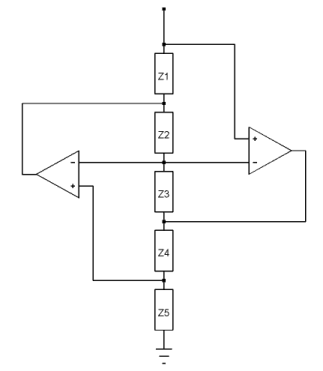
\includegraphics[width=0.35\textwidth]{imagenes/gic.png}
	\caption[Capacitores en un GIC]{Circuito GIC. Si $Z_2$ y $Z_3$ fueran capacitores, no podr\'ian circular las corrientes de bias. Una posible soluci\'on consiste en poner una resistencia en paralelo que permita la circulaci\'on y que sea lo suficientemente grande como para que la impedancia resultante sea aproximadamente capacituva pura.}
	\label{fig:ej_3_GIC}
\end{figure}


Por otro lado, si hay una resistencia $R$ en serie con la entrada del operacional, habr\'a una ca\'ida de tensi\'on $V=I_B^\pm\cdot R$ que puede o no ser despreciable dependiendo de la relaci\'on entre $I_B^\pm$ y $R$ y las caracter\'isticas del circuito. Este efecto es usado en el circuito de medici\'on de $I_B^+$ y $I_B^-$








\subsection{Circuitos con realimentaci\'on}	\label{ssec:realimentacion}

Un circuito realimentado es aquel en el que una proporcion de la salida se redirige a la entrada con el prop\'osito de controlar el comportamiento del sistema. Se  muestra un diagrama de un sistema realimentado t\'ipico en la figura \ref{fig:ej_3_realimentacion}
\footnote{Es com\'un encontrar el mismo modelo con la diferencia que a la entrada se le resta una se\~nal en vez de sumarse. Ambos modelos pueden representar los mismos sistemas (alcanza con cambiar la fase de $\beta$ en 180$^\circ$ para pasar de uno a otro). En este caso se decidi\'o usar la opici\'on con suma ya que es m\'as simple encontrar la similitud con el circuito analizado (ver siagrama de flujo de sen\~nal en la figura \ref{fig:ej_3_signal_flow_consigna_simplificado}}

\begin{description}
	\item[$A_{OL}$:] ganancia a lazo abierto del sistema (\textit{open-loop})
	\item[$A_{CL}$:] ganancia a lazo cerrado del sistema (\textit{closed-loop})
	\item[$A_{CL\,ideal}$:] ganancia a lazo cerrado ideal del sistema. $lim_{T\rightarrow \infty}A_{CL} = A_{CL\,ideal}$
	\item[$\beta$:] ganancia de realimentaci\'on
	\item[$T=A_{OL}\cdot\beta$:] ganancia de lazo
\end{description}

\begin{figure}[htbp] %diagrama realimentacion
	\centering
	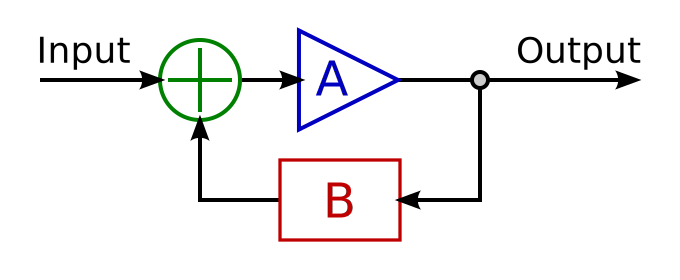
\includegraphics[width=0.5\textwidth]{imagenes/Ideal_feedback_model.png}
	\caption{Diagrama de flujo de se\~nal de sistemas realimentados.}
	\label{fig:ej_3_realimentacion}
\end{figure}


La funci\'on transferencia del sistema H(s) equivale a su ganancia a lazo cerrado:

\[x_d = x_i+x_f\]
\[x_f = \beta x_f\]
\[x_o = A_{OL}x_d = A_{OL}\left( x_i+x_f \right) =  A_{OL}\left( x_i+\beta x_o \right)\]
\[x_o - A_{OL} \beta x_o = A_{OL} x_i\]
\begin{equation}
	\Rightarrow H(s) = A_{CL} = \frac{x_o}{x_i} = \frac{A_{OL}}{1-A_{OL}\beta}
	\label{eq:ej_3_ACL}
\end{equation}

Suponiendo que $T\gg 1$ se obtiene la ganancia a lazo cerrado ideal:
\begin{equation}
	A_{CL\,ideal} = \frac{-1}{\beta}
	\label{eq:ej_3_ACL_IDEAL}
\end{equation}

Un sistema tiene realimentaci\'on negativa si la fase de la ganancia de lazo est\'a entre $180^\circ$ (inclusive) y $360^\circ$ (no inclusive), y realimentaci\'on positiva en caso contrario.

\begin{figure}[htbp] %Ejemplo realimentacion negativa y positiva opamp
	\centering
	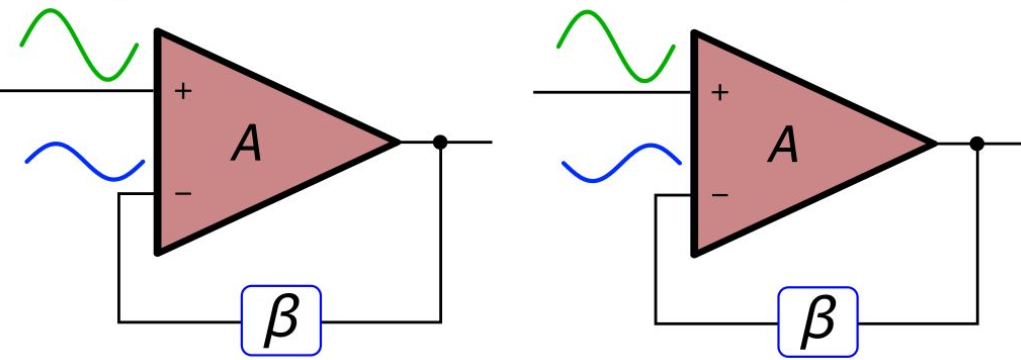
\includegraphics[width=0.5\textwidth]{imagenes/pos_vs_neg_feedback.png}
	\caption{Ejemplo de realimentaci\'on positiva (izquierda) y negativa (derecha) en un \textit{op-amp}.}
	\label{fig:ej_3_realimentacion_pos_vs_neg_opamp}
\end{figure}










\subsection{Funcionamiento del circuito}
La funci\'on del circuito es medir la tensi\'on de offset y las corrientes de bias. La corriente de bias se obtiene midiendo la ca\'ida de tensi\'on que genera sobre una resistencia de $1M\Omega$. En la tabla \ref{tab:ej_3_datasheet} se observan los valores que se esperan medir.


\begin{table}[htbp]
\centering
\begin{tabular}{ccccccc}
               & \multicolumn{3}{c}{TL081}            & \multicolumn{3}{c}{LF356}    \\
\hline              
               & $V_{IO}$(mV) & $I_B$(pA) & $I_O$(pA) & $V_{IO}$(mV) & $I_B$(pA) & $I_O$(pA) \\
\hline
Valor t\'ipico & 3            & 30        & 5         & 3            & 30    & 3     \\
Valor m\'aximo & 6            & 200       & 100       & 10           & 200   & 50   
\end{tabular}
\caption{Valores de las hojas de datos}
\label{tab:ej_3_datasheet}
\end{table}

Todas las tensiones a determinar son amplificadas para as\'i aumentar la precisi\'on en la medici\'on. Se utiliza amplificaci\'on con realimentaci\'on para tener un control preciso sobre la ganancia. En la figura \ref{fig:ej_3_medicion_vio_simple} se muestra un circuito de medici\'on de $V_{IO}$ con ganancia lazo cerrado. Sabiendo que la ganancia de un circuito de amplificacion no inversor es $1+\frac{R_2}{R_1}$, se obtiene $V_{IO}=\frac{R_1}{R_1+R_2}\cdot V_{OUT}$. 


\begin{figure}[htbp]	%medicion vio simplificado
	\centering
	\begin{subfigure}[t]{0.43\textwidth}
		\centering
		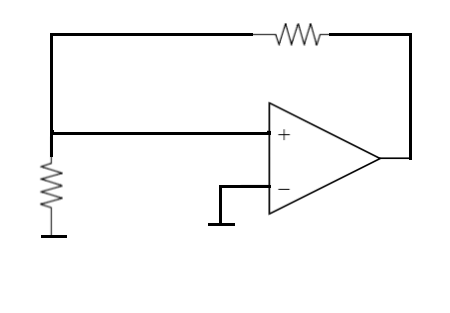
\includegraphics[width=\textwidth]{imagenes/medicion_vio_configuracion_simplificada.png}
		\caption{Con \textit{op-amp} real}
	\end{subfigure}%
	\hfill%%
	\begin{subfigure}[t]{0.43\textwidth}
		\centering
		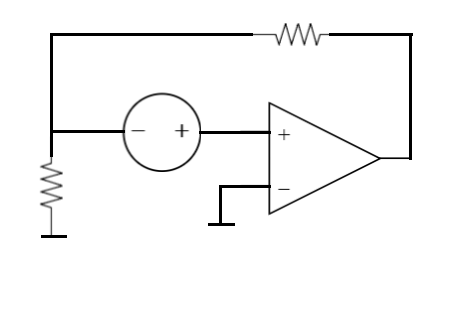
\includegraphics[width=\textwidth]{imagenes/medicion_vio_configuracion_simplificada_opamp_ideal.png}
		\caption{Con \textit{op-amp} ideal y fuente de tensi\'on modelando el \textit{op-amp} real y su tensi\'on de offset}
	\end{subfigure}	
	\caption[Circuito de medici\'on de $V_{IO}$ simplificado.]{Circuito de medici\'on de $V_{IO}$ simplificado.  $V_{OUT} = V_{IO} \cdot \left( 1+ \frac{R_2}{R_1} \right) $. No mide corrientes de bias y amplifica todas las frecuencias por igual.}
	\label{fig:ej_3_medicion_vio_simple}
\end{figure}

Ya que las se\~nales que se quieren medir tienen una amplitud comparable con el ruido que pueda llegar a inducirse en el circuito, es conveniente reducir la amplificaci\'on para las frecuencias mayores a cero. Esto se logra en el circuito presentado en la consigna (figura \ref{fig:ej_3_medicion_vio_consigna})

\begin{figure}[htbp] %medicion vio ib+ ib- posta

	\centering
	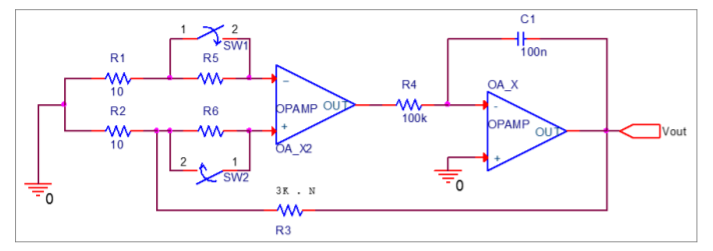
\includegraphics[scale=1]{imagenes/medicion_bias_configuracion_consigna.png}
	\caption{Circuito de medici\'on de $V_{IO}$, $I_B^+$ y $I_B^-$. El dispositivo cuyas caracter\'isticas se miden es el DUT, o \textit{device under test}, el cual es un amplificador con $V_{IO}$ y $I_B$ no despreciables. Las dos resistencias en serie con las entradas del DUT pueden tomar dos valores: $1M\Omega$ o $0\Omega$ si es que se las cortocircuita}
	\label{fig:ej_3_medicion_vio_consigna}
\end{figure}
\begin{figure}[htbp] %medicion vio ib+ ib- posta con opamp ideal
	\centering
	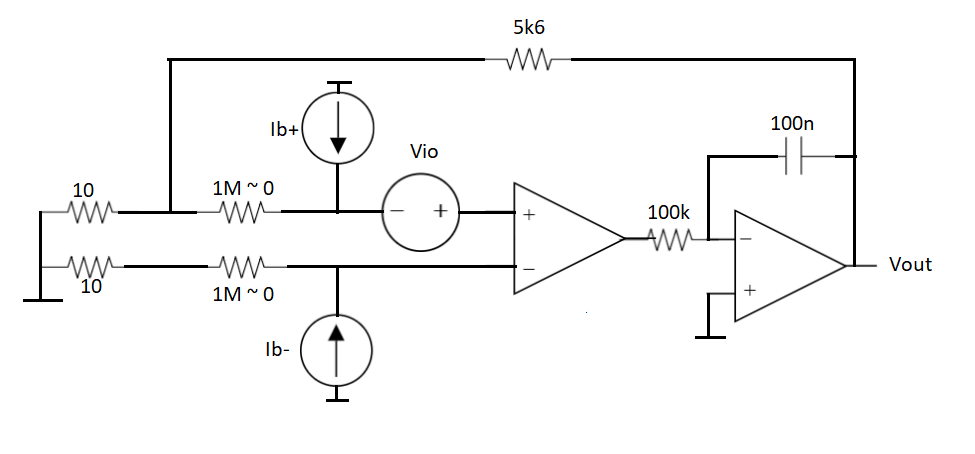
\includegraphics[scale=1]{imagenes/medicion_bias_configuracion_consigna_dos.png}
	\caption{Mismo circuito que en la figura \ref{fig:ej_3_medicion_vio_consigna} cambiando el DUT por el modelo de la figura \ref{fig:ej_3_modelo_opamp_vio_ibias}}
	\label{fig:ej_3_medicion_vio_consigna_modelando}
\end{figure}

Se utiliza un diagrama de flujo de se\~nal (figura \ref{fig:ej_3_signal_flow_consigna_simplificado}) para obtener la funci\'on de transferencia del sistema. Se tomaron la siguiente consideraciones:

\begin{itemize} %consideraciones para el signal flow
	\item $\Delta V_{R1} = I_b^- \cdot 10\Omega \approx 0$
	\item $I_{R2}\approx I_{R3}$
	\item La ganancia a lazo abierto de ambos amplificadores es $A_{vol}$\footnote{Es importante distinguir la ganancia a lazo abierto de un \textit{op-amp} $A_{vol}$ de la ganancia a lazo abierto del circuito total $A_{OL}$ }
	\item La ganancia a lazo cerrado del amplificador que no es el DUT es \[A_{CL} = -\frac{A_{vol}}{1+srC(1+A_{vol})} \approx -\frac{A_{vol}}{1+srCA_{vol}}\] (obtenida en el ejercicio de integrador y derivador).
\end{itemize}


\begin{figure}[htpb]%signal flow consigna
	\centering
	\begin{subfigure}[t]{0.45\textwidth}
		\centering
		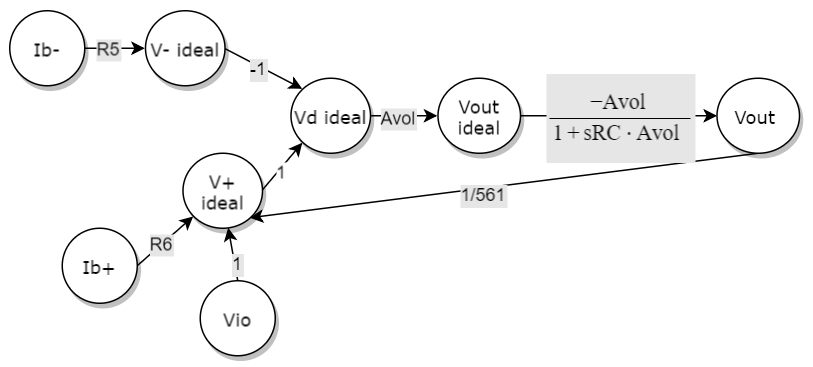
\includegraphics[width=\textwidth]{imagenes/signal_flow_consigna.png}
		\caption{Diagrama de flujo de se\~nal para el circuito de la consigna usando el modelo de la figura \ref{fig:ej_3_modelo_opamp_vio_ibias} para el DUT. Se desprecian los efectos de $I_B$ y $V_{IO}$ en el otro \textit{op-amp}.}
		\label{fig:ej_3_signal_flow_consigna_no_simplificado}
	\end{subfigure}%
	\hfill%%
	\begin{subfigure}[t]{0.45\textwidth}
		\centering
		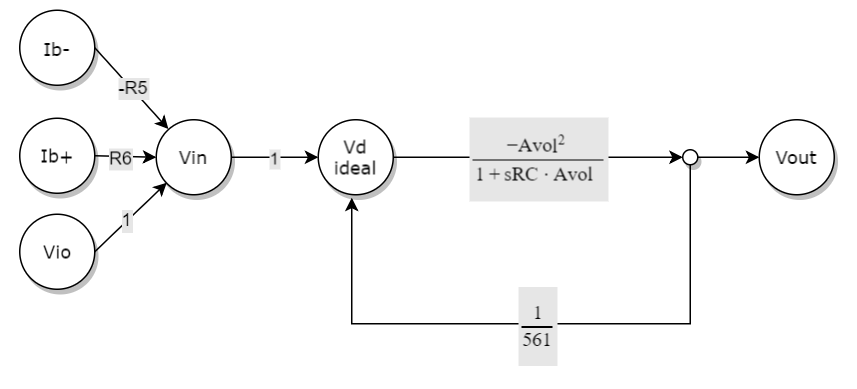
\includegraphics[width=\textwidth]{imagenes/signal_flow_consigna_simplificado.png}
		\caption{Simplificaci\'on del diagrama de flujo de se\~nal. La estructura coincide con la de un circuito con realimentacion (ver figura \ref{fig:ej_3_realimentacion}). }
		\label{fig:ej_3_signal_flow_consigna_simplificado}
	\end{subfigure}
	\label{fig:ej_3_signal_flow_consigna}
	\caption{}	
\end{figure}


El diagrama de flujo de se\~nal coincide con el de un sistema realimentado descripto en la secci'on \ref{ssec:realimentacion}. La \'unica diferencia es que en este caso la entrada no es una \'unica se\~nal sino una suma:

\begin{equation}
	V_{in} = V_{IO} + I_B^+\cdot R6 - I_B^-\cdot R5
	\label{eq:ej_3_vin_aparente}
\end{equation}

Cabe destacar $V_{in}$ es una forma abstracta de agrupar los efectos no ideales del \textit{op-amp} real, y no corresponde necesariamente con una diferencia de potencial real entre dos puntos.

 Se puede obtener entonces la ganancia de lazo cerrado y la ganancia de realimentaci\'on del circuito:
\[\beta = \frac{1}{561}\]
\[A_{OL} = -\frac{A_{vol}^2}{1+sRC\cdot A_{vol}}\]

Con estos valores y teniendo en cuenta la ecuaci\'on \ref{eq:ej_3_ACL} se obtiene la funci\'on transferencia del sistema:

\begin{equation}
	H(s)=\frac{-\frac{A_{vol}^2}{1+sRC\cdot A_{vol}}}{1+\frac{A_{vol}^2}{1+sRC\cdot A_{vol}}\beta}
	=-\frac{1}{\frac{1}{A_{vol}^2}+\beta}\cdot \frac{1}{\frac{s}{\frac{1+A_{vol}^2\beta}{RCA_{vol}}} +1}
	\label{eg:ej_3_transferencia_consigna_sin_simplificar}
\end{equation}


Si se considera que $A_{vol}^2\beta \gg 1 \Rightarrow \beta \gg \frac{1}{A_{vol}^2}$ se puede simplificar la expresi\'on:



	\[H(s) = -\frac{1}{\beta}\cdot \frac{1}{\frac{s}{\frac{A_{vol}\beta}{RC}}+1}\]


Utilizando el modelo de $A_{vol}$ de polo dominante (explicado en detalle en el ejercicio 1), se obtiene:
\[H(s) = -\frac{1}{\beta} \cdot \frac{1}{\frac{s}{\frac{\frac{A_o}{\frac{1}{\omega _p}+1}\beta}{RC}}+1} \]

\begin{equation}
	H(s) = -\frac{1}{\beta} \cdot \frac{1}{s^2\frac{RC}{w_pA_o\beta}+s\frac{RC}{A_o\beta}+1}
	\label{eq:ej_3_transferencia_consigna_simplificada}
\end{equation}



Sabiendo que $lim_{T\rightarrow \infty}A_{CL} = A_{CL\,ideal}$:

\begin{equation}
	A_{CL\,ideal} = -\frac{1}{\beta} = -561
\end{equation}


\subsubsection{Funcionamiento en DC: mediciones de $V_{IO}$ y $I_B$}

Cuando $f=0$, evaluando en la funci\'on transferencia (ecuaci\'on \ref{eg:ej_3_transferencia_consigna_sin_simplificar}) se obtiene que la ganancia del circuito es $-\frac{1}{\beta}=-561$, por lo que $V_{in}=-\frac{V_{out}}{561}$


\begin{description}%mediciones tomadas
	\item[Medici\'on de $V_{IO}$:] Cortocircuitando las resistencias R5 y R6 se obtiene que $V_{in} = V_{IO}$, valor que se puede obtener midiendo $V_{OUT}$:
	
	\[V_{IO} = -\frac{V_{OUT}}{561}\]
	\item[Medici\'on de $I_B^\pm$ y $I_B$:] Cortocircuitando R5 se obtiene $-\frac{V_{OUT}}{561} = V_{IO} + I_B^+\cdot R6$. Despejando:
	\[I_B^+=\frac{1}{R6}\cdot\left( -\frac{V_{OUT}}{561}-V_{IO}  \right) \]
	An\'alogamente,
	\[I_B^-=-\frac{1}{R5}\cdot \left( V_{IO} + \frac{V_{OUT}}{561}   \right)\]
	Una vez obtenidas $I_B^\pm$, se calcula $I_B$ definida como $\frac{I_B^++I_B^-}{2}$
\end{description}

\begin{table}[htbp]%resultados
\centering
\begin{tabular}{ccccc}
                       & \multicolumn{2}{c}{TL081} & \multicolumn{2}{c}{LF356} \\
\hline
Par\'ametro a calcular & $V_{OUT}$(mV)& Resultado  & $V_{OUT}$(mV)& Resultado  \\
\hline
$V_{IO}$               & 255          & -0,455mV   & 135          & -0,241mV   \\
$I_B^+$                & 0,675        & 453pA      & 0,179        & 241pA      \\
$I_B^-$                & 202          & -94,5pA    & 207          & -143pA     \\
$I_{IO}$			   &     ---      & 584 pA	   &	  ---     & 384pA      \\
$I_B$				   &     ---      & 179 pA     &      ---     & 49pA
\end{tabular}%

\caption{Resultados}
\label{tab:ej_3_resultados}
\end{table}

Las mediciones que son acordes a lo especificado en la hoja de datos son $V_{IO}$  y $I_B$ en los dos amplificadores. Por otro lado, se midieron valores de $I_O$ mayores al m\'aximo especificado por el fabricante, tambi\'en en los dos casos.



\subsubsection{Funcionamiento en AC}

\begin{table}[htbp]
\centering
\begin{tabular}{ccllcll}
                   & \multicolumn{3}{c}{TL081}         & \multicolumn{3}{c}{LF356}          \\
\hline
$\omega _p$ (rad/s) & \multicolumn{3}{c}{$2\pi \cdot 94$} & \multicolumn{3}{c}{$2\pi \cdot 157$} \\
$A_o$ (V/mV)       & \multicolumn{3}{c}{200}           & \multicolumn{3}{c}{200}           
\end{tabular}
\caption{Caracter\'isticas de los amplificadores}
\label{tab:ej_1_}
\end{table}


La transferencia (ecuaci\'on \ref{eq:ej_3_transferencia_consigna_simplificada}) cumple con la forma 
\[\frac{C(cte)}{\frac{s^2}{\omega_0^2}+s\frac{2\xi}{\omega_0}+1}\]

Se obtiene
\[\omega _0 = \sqrt{\frac{\omega_pA_o\beta}{RC}}\]
\[\xi=\frac{1}{2}\,\sqrt{\frac{\omega_pA_o\beta}{RC}}\,\frac{RC}{A_o\beta}=\frac{1}{2}\,\sqrt{\frac{\omega_pRC}{A_o\beta}}\]


con polos en el semiplano izquierdo del plano complejo (ver secci\'on \ref{ssec:ej_3_estabilidad_consigna}). Esto indica que el circuito es un pasabajos de orden 2 con frecuencia de corte $f_0=\frac{1}{2\pi}\cdot \sqrt{\frac{\omega_pA_o\beta}{RC}}=$. Para el TL081, $f_0=291Hz$ y para el LF356 $f_0=376Hz$. Se encontr\'o experimentalmente que el mayor ruido era de 50Hz. Si para atenuarlo se decidiera poner la frecuencia de corte a menos de 50Hz, se necesitar\'ia como m\'inimo un capacitor de $C=\frac{1}{4\pi^2}\cdot \frac{\omega_pA_o\beta}{R(50Hz)^2}$. Para el TL081, $C>0,5\mu F$ y para el LF356 $C>0,9 \mu F$.

Para el LF356, $xi = 0.033$ y para el TL081, $xi = 0,026$, por lo tanto ambos tienen sobrepico. Por este motivo, no alcanza con que $f_0<50Hz$ para asegurar que se est\'a atenuando la interferencia a esta frecuencia. Por el contrario: si $f_0$ es menor que 50Hz pero cercano, puede ser que caiga dentro del sobrepico y se est\'e amplificando.





\subsection{Estabilidad en diferentes configuraciones} 

Para determinar la estabilidad del circuito se analizan la posici\'on de los polos de la funci\'on transferencia:

\subsubsection{Configuraci\'on consigna} \label{ssec:ej_3_estabilidad_consigna}
De la ecuaci\'on \ref{eq:ej_3_transferencia_consigna_simplificada} se obtienen los polos.

Los polos de la funci\'on transferencia tienen la forma 
\[s_{1,2} = \frac{-\frac{2\xi}{\omega_0}\pm\sqrt{\frac{4\xi^2}{\omega_0^2}-\frac{4}{\omega_0^2}}}{\frac{2}{\omega_0^2}}\]

\[=-\omega_0\xi \pm \frac{1}{\omega_0}\sqrt{\xi^2-1}\]

Como $\xi<0$, el segundo t\'ermino es imaginario y la parte real del los polos es $-\omega_0\xi<0$. Por lo tanto, el sistema es estable.


\subsubsection{Otras configuraciones}

Si se invierten las entradas de alguno de los amplificadores, el diagrama de flujo de se\~nal sufre leves modificaciones:


\begin{figure}[h]%signal flow invirtiendo noDUT
	\centering
	\begin{subfigure}[t]{0.49\textwidth}
		\centering
		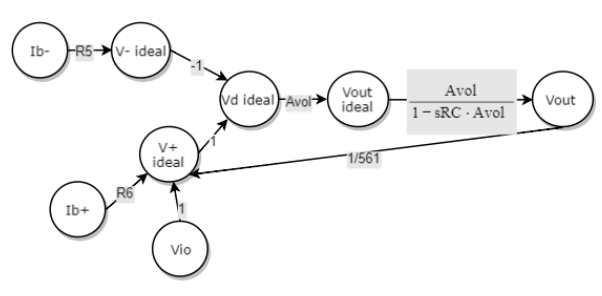
\includegraphics[width=\textwidth]{imagenes/signal_flow_inv_noDUT.png}
		\caption{}
		\label{fig:ej_3_signal_flow_inv_noDUT_no_simplificado}
	\end{subfigure}%
	\hfill%%
	\begin{subfigure}[t]{0.49\textwidth}
		\centering
		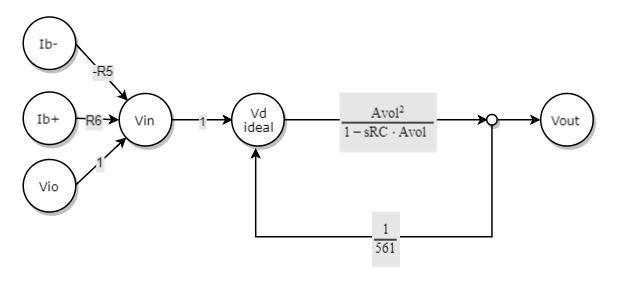
\includegraphics[width=\textwidth]{imagenes/signal_flow_inv_noDUT_simplificado.png}
		\caption{}
		\label{fig:ej_3_signal_flow_inv_noDUT_simplificado}
	\end{subfigure}
	\caption{Diagrama de flujo de se\~nal el circuito de la consigna invirtiendo las entradas en el amplificador no DUT. La obtenci\'on de la transferencia del amplificador no DUT es an\'aloga a la de la configuraci\'on no inversora usado en el circuito de la consigna}
	\label{fig:ej_3_signal_flow_inv_noDUT}	
\end{figure}


\begin{figure}[h]%signal flow invirtiendo ambos
	\centering
	\begin{subfigure}[t]{0.49\textwidth}
		\centering
		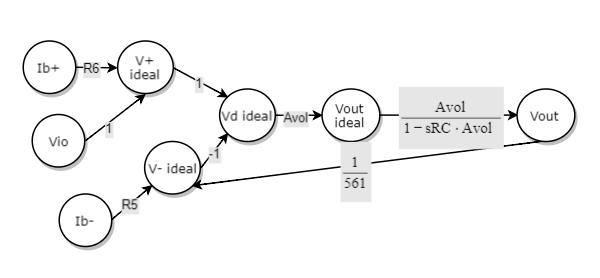
\includegraphics[width=\textwidth]{imagenes/signal_flow_inv_ambos.png}
		\caption{}
		\label{fig:ej_3_signal_flow_inv_ambos_no_simplificado}
	\end{subfigure}%
	\hfill%%
	\begin{subfigure}[t]{0.49\textwidth}
		\centering
		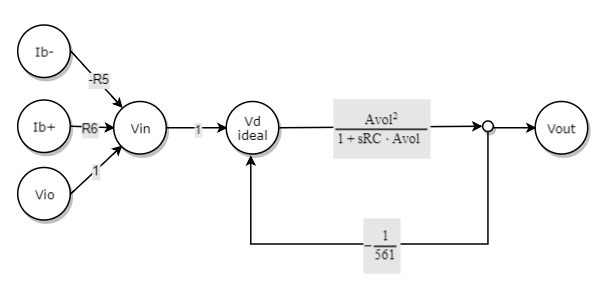
\includegraphics[width=\textwidth]{imagenes/signal_flow_inv_ambos_simplificado.png}
		\caption{}
		\label{fig:ej_3_signal_flow_inv_ambos_simplificado}
	\end{subfigure}
	\label{fig:ej_3_signal_flow_inv_ambos}	
	\caption{Diagrama de flujo de se\~nal el circuito de la consigna invirtiendo las entradas en ambos amplificadores.}
\end{figure}

El c\'alculo de la estabilidad en estas configuraciones es igual al ya realizado con el circuito de la consigna: se obtiene la ganancia a lazo abierto y la ganancia de realimentaci\'on del diagrama, con la ecuaci\'on \ref{eq:ej_3_ACL} se calcula la transferencia (teniendo en cuenta el modelo de polo dominante de $A_{vol}$ ) y luego se analiza la posici\'on de los polos en el plano complejo (es estable si est\'an en el semiplano negativo).


\end{document}
